\section{Gaussian Graphical Models}

In this chapter, we study problems related to submodel selection in Gaussian graphical models. In Section \ref{sec-prelim}, we begin by defining graphical models and Gaussian graphical models. We then study the existence and computation of the maximum likelihood estimator of the precision matrix in a Gaussian graphical model under different assumptions on the graph. In Section \ref{sec-hyp-test}, we apply the $p^*$ approximation from Section \ref{sec-pstar} to compute an accurate approximation for submodel testing. The test resulting from this approximation is then numerically evaluated against the likelihood ratio test in different dimensionality settings.

\subsection{Preliminaries}

We start by a brief introduction to elementary concepts in graph theory that will be useful in the rest of this chapter. Let $\G = (\Gamma, E)$ be a graph with nodes $\Gamma$ and edges $E \subset \Gamma \times \Gamma$. For convenience, we will assume that the nodes are numbered and use  $\G = ([p], E)$ and $E \subset [p] \times [p]$ for $p = |\Gamma|$.  We denote by $\t{bd}(i)$ the set of \textit{neighbours} of $i \in [p]$, that is $\t{bd}(i) = \eset{ j \in [p] : \eset{i, j} \in E \t{ and } j \neq i}$. The graphs under study in this thesis will be unconnected and won't contain any loop. This lets us write edges using the set notation $e = \eset{i, j}$ for $e \in E$. However, it will sometimes be useful to treat the set of edges as a set of indices on a matrix. In this case, we will need to introduce the \textit{augmented edge set} to include indices refering to the diagonal entries of the matrix. The augmented edge set $E^*$ of $E$ is constructed by adding all possible loop in $\G$, $E^* = E \cup \eset{ \eset{i} : i \in \Gamma }$.

A graph $\G$ is said to be \textit{complete} if all pairs of distinct nodes are connected by an edge. A set of nodes $C \subset [p]$ is called a \textit{clique} if the subgraph $\G_C = (C, E_C)$ with $E_C = \eset{ \eset{i, j} \in E : \eset{i, j} \subset C }$ is complete. We call $\c{C}(\G)$ the set of cliques in $\G$.

An important class of graphs are \textit{chordal graphs}. A chordal graph $\G$ is a graph in which each cycle of length at least 4 has a \textit{chord}, which is an edge which is not part of the cycle connecting two nodes in the cycle.

As mentioned before, edges will be used to index matrices. If $\G = ([p], E)$, and $M \in \R^{p \times p}$, we introduce the following notation:
\begin{itemize}
    \item If $e = \eset{i, j} \in E$, then $M_e = M_{ij}$;
    \item If $A, B \subset [p]$, then $M_{A, B}$ is the $|A| \times |B|$ matrix construced by keeping rows labeled by the entries in $A$ and columns labeled by entries in $B$;
    \item If $C \subset [p]$, then $M_C = M_{C, C}$;
    \item {
        If $A, B \subset [p]$, then $[M_{A, B}]^{[p]}$ is the $p \times p$ matrix with entries satisfying 
        \begin{equation*}
            [M_{A, B}]^{\Gamma}_{ij} = \begin{cases}
                M_{ij} \ \t{ if } \eset{i, j} \in A \times B, \\
                0 \ \ \ \ \ \t{otherwise}.
            \end{cases}
        \end{equation*}
    }
\end{itemize}
Since most matrices manipulated will be referencing quantities related to nodes in a graph, indexing of matrices and derived matrices will be done with respect to the nodes of the graph instead of row or column number of a matrix. For instance, if $A, B \subset [p]$ and $M \in \R^{p \times p}$, using the notation we just introduced, we have
\begin{equation*}
    (M_{A, B})_{ab} = M_{ab} \ \ \t{for all } a \in A, b \in B.
\end{equation*}

\subsection{Maximum likelihood estimation in Gaussian graphical models}

A graphical model is a probabilistic model associating relations between random variables to a graph. The random variables of the model are represented by nodes in the graph and conditional independence relations are represented by missing edges between the corresponding nodes of the graph.

Consider a random vector $X$ distributed according to the \textit{multivariate Gaussian} distribution $N_p(0, \Omega^{-1})$, where $\Omega \in \S^p_{\succ 0}$, called the \textit{precision matrix}, is the inverse of the covaraince matrix $\Sigma$. Thus, the density of $X$ is
\begin{equation} \label{eq-density-gaussian}
    f(x; \Omega) = (2\pi)^{-p/2} |\Omega|^{1/2} \expfc{-\frac{1}{2} \trB{xx^\top \Omega} }.
\end{equation}
Clearly, the multivariate Gaussian distribution is an exponential family with canonical parameter $\Omega$ and sufficient statistic $\frac{1}{2}xx^\top$. We start by stating a result about multivariate Normal distribution that can be found in \cite[Proposition C.5]{lauritzen1996}. 

\begin{lemma} \label{lem-gaussian-cond}
    Let $X \sim N_p(\mu, \Sigma)$ and $A, B \subset [p]$ be disjoint. Then, the conditional distribution of $X_A$ given $X_B = x_B$ is $N_{|A|}(\mu_{A|B}, \Sigma_{A|B})$ where
    \begin{align*}
        \mu_{A|B} = \mu_A + \Sigma_{A,B}\Sigma^{-1}_{B,B}(x_B - \mu_B) && \t{and} && \Sigma_{A|B} = \Sigma_{A,A} - \Sigma_{A,B}\Sigma^{-1}_{B,B}\Sigma_{B,A}.
    \end{align*} 
    One recognizes that the conditional covariance matrix $\Sigma_{A|B}$ is the Schur complement of $\Sigma_B$ in $\Sigma$.
\end{lemma}

We parametrize the multivariate Normal distribution in terms of the precision matrix because of its special role in the context of graphical models. Indeed, the conditional independence relations of the entries a random vector $X \sim N_p(0, \Omega)$ are characterized by the sparsity patterns of the precision matrix $\Omega$. This is shown in the following lemma from \cite[Proposition 5.2]{lauritzen1996}.
\
\begin{lemma}
    Let $X \sim N_p(\mu, \Sigma)$ and let $i, j \in [p]$ with $i \neq j$. Then
    \begin{equation} \label{eq-lemma-markov}
        \Omega_{ij} = 0 \iff X_i \independent X_j | X_{[p] \setminus \eset{i,j}}.
    \end{equation}
\end{lemma}
\begin{proof}
    By Lemma \ref{lem-gaussian-cond}, we have that the bivariate vector $X_{\eset{i,j}}$ is Gaussian with covariance matrix $\Sigma_{\eset{i,j}|[p]\setminus\eset{i,j}}$ equal to the Schur complement of $\Sigma_{[p] \setminus \eset{i,j}}$. The statement in (\ref{eq-lemma-markov}) is thus equivalent to 
    \begin{equation*}
        \Omega_{ij} = 0 \iff \Sigma_{\eset{i,j}|[p]\setminus\eset{i,j}}\ \t{is diagonal}.
    \end{equation*}
    Using the Schur complement inverse property, we have that
    \begin{equation*}
        \Sigma_{\eset{i,j}|[p]\setminus\eset{i,j}} 
        = \left[\Omega_{\eset{i,j}}\right]^{-1} 
        = \begin{pmatrix}
            \Omega_{ii} & \Omega_{ij}\\
            \Omega_{ji} & \Omega_{jj}
            \end{pmatrix}^{-1}
        = \frac{1}{|\Omega_{\eset{i,j}}|} \begin{pmatrix}
            \Omega_{jj} & -\Omega_{ij}\\
            -\Omega_{ji} & \Omega_{ii} 
            \end{pmatrix}^{-1}.
    \end{equation*}
    Hence, $\Sigma_{\eset{i,j}|[p]\setminus\eset{i,j}}$ is diagonal if and only if $\Omega_{ij} = 0$, completing the proof of the lemma.
\end{proof}

Consider a graph $\G = ([p], E)$. We say that $X$ satisfies the \textit{Gaussian graphical model} with graph $\G$ if $X \sim N_p(0, \Omega)$ and
\begin{equation} \label{eq-ggm}
    \Omega_{i j} = 0 \t{ for all } \eset{i,j} \notin E^*.
\end{equation}
Property (\ref{eq-ggm}) corresponds to the pairwise Markov property in graphical model theory \cite{lauritzen1996}. Note that the independence relations of the entries of $X$, the connectivity of the nodes in $\G$ and the sparsity pattern of $\Omega$ are all the same concept viewed from a different angle, which each on its own will help in studying them.

We now study properties of the maximum likelihood estimator in a Gaussian graphical model, largely following the presentation of Uhler \cite[Section 9]{maathuis2018handbook}.

Consider a sample $X = (X_1, \ldots, X_n)$ from a Gaussian distribution. The log-likelihood function for a precision matrix $\Omega \in \S^p_{\succ 0}$ obtained from (\ref{eq-density-gaussian}) is
\begin{equation*}
    \ell(\Omega; X) = \frac{n}{2} \log |\Omega| - \frac{1}{2}\tr[XX^\top\Omega].
\end{equation*}
Rewriting the log-likelihood in terms of the sufficient statistic $S = n^{-1}XX^\top$, we get that
\begin{equation} \label{eq-likelihood}
    \ell(\Omega; S) = \frac{n}{2}\log |\Omega| - \frac{n}{2}\tr[S\Omega].
\end{equation}
In the \textit{saturated model} where no constraints are put on the entries of $\Omega$, the maximum likelihood estimator is defined when $S \in S^p_{\succ 0}$ and is equal to
\begin{equation*}
    \hat\Omega = S^{-1}.
\end{equation*}
Remark that, if we are interested in estimating the maximum likelihood estimator $\hat\Omega$ of a Gaussian graphical model with graph $\G = ([p], E)$, the solution $\hat\Omega$ must lie in the subset $\S_{\succ 0}(\G)$ of $\S^p_{\succ 0}$ in which the conditional independence relations encoded in $\G$ are satisfied. We are now left with the following optimization problem
\begin{align} \label{eq-primal}
    \begin{split}
        &\underset{\Omega \in \S^p_{\succ 0}}{\t{maximize}}\ \  \log |\Omega| - \tr[S\Omega]\\
        &\t{subject to}\ \ \Omega \in \S(\G).
    \end{split}
\end{align}
Since the Gaussian graphical model condition is a linear constraint, the set $\S(\G)$ is a convex cone. Showing that the objective function in (\ref{eq-primal}) is concave would imply that maximum likelihood estimation in Gaussian graphical models is a convex optimization problem. This would allow us to bring new insights to the maximum likelihood problem by studying its dual formulation. The following lemma from \cite[Proposition 9.2.1]{maathuis2018handbook} states that the objective function is indeed concave.
\begin{lemma}
    The function $f : \S^p_{\succ 0} \rightarrow \R, X \mapsto \log |X| - \trB{SX}$ is concave.
\end{lemma}
\begin{proof}
    Remark thath the sum of a concave function and a linear function is concave, and $\trB{SX}$ is linear in $X$. Thus, it is sufficient to show that the logarithm of the determinant of a matrix is concave. To show this, we consider the line $\eset{ U + tV : t \in \R }$ for $U, V \in \S^p_{\succ 0}$. We show that $X \mapsto \log |X|$ is concave on $\S^p_{\succ 0}$ by proving that $g(t) = \log |U + tV|$ is concave as follows. Since $U \in \S^p_{\succ 0}$, both $U^{1/2}$ and $U^{-1/2}$ exist and we have 
    \begin{align*}
        g(t)
        &= \log |U + tV| \\
        &= \log |U^{1/2}(1_p + tU^{-1/2}VU^{-1/2}|\\
        &= \log |U| + \log |1_p + tU^{-1/2}VU^{-1/2}|.
    \end{align*}
    Let $\lambda_i$ be the eigenvalues of $U^{-1/2}VU^{-1/2}$ and note that the eigenvalues of $1_p + tU^{-1/2}VU^{-1/2}$ are $1 + t\lambda_i$. Therefore
    \begin{equation*}
        g(t) = \log |U| + \sum_{i=1}^p \log (1 + t\lambda_i).
    \end{equation*}
    Now, since each $\log (1 + t\lambda_i)$ is concave in $t$, we have that $g$ is concave, which completes the proof of the lemma.
\end{proof}

We can now study the dual problem to (\ref{eq-primal}). The Lagragian of the likelihood maximization problem in Gaussian graphical models is given by
\begin{align*}
    \mathcal{L}(\Omega, \nu)
    &= \log |\Omega| - \tr[S\Omega] - 2 \sum_{\eset{i, j} \notin E} \nu_{ij}\Omega_{ij}\\
    &= \log |\Omega| - \sum_{i=1}^p S_{ii}\Omega_{ii} - 2 \sum_{\eset{i,j} \in E} S_{ij}\Omega_{ij} - 2 \sum_{\eset{i, j} \notin E} \nu_{ij}\Omega_{ij}
\end{align*}
The Lagrange dual $H$ of (\ref{eq-primal}) is given by $H(\nu) = \mathcal{L}(\Omega^\nu, \nu)$ where $\Omega^\nu$ is the maximizer of $\mathcal{L}(\Omega, \nu)$. Let $\Omega^\nu$ be the maximizer of $\mathcal{L}(\Omega, \nu)$ with respect to $\Omega$. Then, the inverse $\Sigma^\nu$ of $\Omega^\nu$ satisfies the following
\begin{equation*}
    \Sigma^\nu_{ij} = \begin{cases}
        S_{ij}\ \t{ if } i = j \t{ or } \eset{i, j} \in E\\
        \nu_{ij}\ \t{otherwise}.
    \end{cases}
\end{equation*}
Note that $\Sigma^\nu$ is the matrix formed by replacing entries in $S$ corresponding to missing edges with entries of the dual variables $\nu_{ij}$. Replacing $\Omega^\nu$ in the expression for the Lagrange dual function $H$, we obtain that
\begin{align*}
    H(\nu) 
    = \c{L}(\Omega^\nu, \nu)
    &= \log |\Omega^\nu| - \tr[S\Omega^\nu] - 2 \sum_{\eset{i, j} \notin E} \nu_{ij}\Omega^\nu_{ij}\\
    &= \log |\Omega^\nu| - \tr[\Sigma^\nu\Omega^\nu] + 2 \sum_{\eset{i, j} \notin E} \Sigma^\nu_{ij}\Omega^\nu_{ij} - 2 \sum_{\eset{i, j} \notin E} \nu_{ij}\Omega^\nu_{ij}\\
    &= \log |\Omega^\nu| - p = -\log |\Sigma^\nu| - p.
\end{align*}
Hence the dual to (\ref{eq-primal}) is
\begin{align} \label{eq-dual}
    \begin{split}
        &\underset{\Sigma \in \S^p_{\succ 0}}{\t{minimize}}\ \  -\log |\Sigma| - p\\
        &\t{subject to}\ \ \Sigma_{ij} = S_{ij}\ \t{ for all } i = j \t{ or } \eset{i, j} \in E
    \end{split}
\end{align}
To prove that problems (\ref{eq-primal}) and (\ref{eq-dual}) are equivalent, we must show that strong duality holds for this convex optimization problem. By \textit{Slater's constraint quantification} \cite[Section 5.3.2]{boyd2004convex}, it is enough to show that there exists an $\Omega^* \in \S^p_{\succ 0}$ that is strictly feasable for the primal problem. Since the identity matrix is positive definite and is an element of $\S(\G)$ for any $\G$, strong duality holds for any graph $\G$. Thus, can freely study both formulations of the optimization problem. Furthermore, problems (\ref{eq-primal}) and (\ref{eq-dual}) have a solution if and only if $\log |\Sigma| + p$ is unbounded from above in the set of feasable matrices. We have yet to study under which condition this is the case.

To that end, let us first introduce some notation. Let $\G = ([p], E)$ and $\Sigma \in \R^{p\times p}$, the \textit{$\G$-partial matrix} $\Sigma^\G$ of $\Sigma$ is the partial matrix contructed by removing entries in $\Sigma$ corresponding to missing edges in $\G$, see Figure \ref{fig-no-completion} for an example. With this notation, the dual problem (\ref{eq-dual}) can be reformulated as follows,
\begin{align} \label{eq-completion}
    \begin{split}    
        &\underset{\Sigma \in \S^p_{\succ 0}}{\t{minimize}}\ \  -\log |\Sigma| - p\\
        &\t{subject to}\ \ \Sigma^\G = S^\G.
    \end{split}
\end{align}
In this formulation, the dual optimization problem corresponds to a \textit{positive definite matrix completion} problem in which the matrix $\Sigma$ is partially specified from entries of the sample covariance matrix corresponding to edges present in $\G$. Furthermore, Uhler \cite[Section 9.4]{maathuis2018handbook} presents a geometric argument tying together the matrix completion to the original convex optimization formulation of the likelihood maximization problem.

\begin{theorem}
    Consider a Gaussian graphical model associated to the graph $\G$ and a sample covariance matrix $S$. The maximum likelihood estimation problems have unique solutions $\hat\Omega$ and $\hat\Sigma$ if and only if $S^\G$ has a positive definite completion. In this case, $\hat\Sigma$ is the positive definite completion of $S^\G$ and $\hat\Omega = \hat\Sigma^{-1}$.
\end{theorem}
\begin{proof}
    This theorem is a reformulation of \cite[Theorem 9.4.2]{maathuis2018handbook} in which $\c{L} \cap \S^p_{\succ 0} = \S(\G)$, which we have shown to contain at least $1_p$.
\end{proof}

We now study the existence of a solution to the maximum likelihood question by finding the conditions under which a $\G$-partial sample covariance matrix can be completed to a positive definite matrix. Gross et al.\,\cite{10.3150/16-BEJ881} introduce the \textit{maximum likelihood threshold} of a graph $\G$. The maximum likelihood treshold of a graph $\G$, denoted by $\t{mlt}(\G)$, is the smallest number of data points that guarantees the maximum likelihood estimator  to exist almost surely in a Gaussian graphical model associated to the graph $\G$. In other words, $\t{mlt}(\G)$ is the smallest number of observations for which $S^\G$ can be completed to a positive definite matrix. For a Gaussian graphical model over $p$ variables, the rank of the sample covariance constructed from a sample of $n$ observations is $\t{rank}(S) = \min(n, p)$. Hence, if $n \geq p > 0$, $S$ itself is a valid positive completion of $S^\G$, giving the worst case bound
\begin{equation} \label{eq-pessimistic-mlt}
    \t{mlt}(\G) \leq p,
\end{equation}
where equality holds if $\G$ is complete.

A necessary condition for a solution to the matrix completion problem to exist, is that all completely specified principal submatrices $S^\G_{[p]\setminus I}$ of $S^\G$ for $I \subset [p]$ must be positive definite. The principal submatrix $S^\G_{[p]\setminus I}$ of $S^\G$ is completely specified if it contains no missing value. The necessary condition can be shown by the following argument. Let $S^\G_{[p]\setminus I}$ be a principal completely specified submatrix of $S^\G$ such that there exists $z \in \R^{p-|I|}\setminus \eset{0}$ with $z^\top S^\G_{-I} z \leq 0$. Then if $S^\G_+$ is the positive definite completion of $S^\G$, it holds that $x^\top S^\G_+ x \leq 0$ for $x \in \R^p \setminus \eset{0}$ with $x_I = z$ and $x_{-I} = 0$, contradicting the positive definiteness of $S^\G_+$. Furthermore, if $C$ is a clique of $\G$, $C$ is complete and thus the submatrix $S^\G_C$ is a completely specified principal submatrix of $S^\G$. As $S^\G_C$ is complete, it is positive definite with probability one if and only if $n \geq |C|$. Now let $q(\G) = \max \eset{|C| : C \t{ is a clique of } \G}$ be the maximum clique size in $\G$. We can then lower bound the maximum likelihood threshold by
\begin{equation} \label{eq-mlt-upper-bound}
    q(\G) \leq \t{mlt}(\G).
\end{equation}


\begin{figure}[!tbp]
    \begin{minipage}[c]{.3\linewidth}
        \centering
        \begin{gather*}
            \begin{pmatrix}
                1 & 0.9 & 0.3 & -0.9 \\
                0.9 & 1 & 0.9 & -0.7 \\
                0.3 & 0.9 & 1 & 0.9 \\
                -0.9 & -0.7 & 0.9 & 1
            \end{pmatrix}\\
            S
        \end{gather*}
    \end{minipage}
    \hfill
    \begin{minipage}[c]{.2\linewidth}
        \centering
        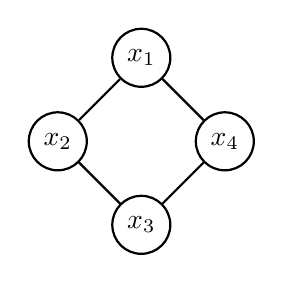
\begin{tikzpicture}[node distance={15mm}, thick, main/.style = {draw, circle}] 
            \node[main] (1) {$x_1$}; 
            \node[main] (2) [below left of=1] {$x_2$};
            \node[main] (3) [below right of=2] {$x_3$}; 
            \node[main] (4) [above right of=3] {$x_4$};
            \draw (1) -- (2);
            \draw (2) -- (3);
            \draw (4) -- (3);
            \draw (1) -- (4);
        \end{tikzpicture}
    \end{minipage}
    \hfill
    \begin{minipage}[c]{.3\linewidth} %inequalities
        \centering
        \begin{gather*}
             \begin{pmatrix}
                1 & 0.9 & ? & -0.9 \\
                0.9 & 1 & 0.9 & ? \\
                ? & 0.9 & 1 & 0.9 \\
                -0.9 & ? & 0.9 & 1
            \end{pmatrix}\\
            S^\G
        \end{gather*}
    \end{minipage}

    \caption{Example from \cite[Section 9.3]{maathuis2018handbook} of a matrix $S$ for which all completely specified submatrices of $S^\G$ are positive definite but which doesn't have a positive definite completion.}
    \label{fig-no-completion}
\end{figure}

However, as shown in the example in Figure \ref{fig-no-completion}, this condition is not sufficient for the existence of a positive definite completion. Still, Grone et al. \cite{GRONE1984109} show that this condition is also sufficient if and only if $\G$ is a chordal graph.
\begin{theorem} \label{thm-chordal-iff}
    For a graph $\G$, the following statements are equivalent.
    \begin{enumerate}[i.]
        \item A partial matrix $M^\G$ has a positive definite completion if and only if all completely specified submatrices of $M^\G$ are positive definite.
        \item $\G$ is chordal.
    \end{enumerate}
\end{theorem}
A consequence of this theorem is that if $\G$ is a chordal graph, then $\t{mlt}(\G) = q(\G)$. This result for chordal graphs can be used to compute an upper bound on the maximum likelihood treshold of a general graph tighter than the worst-case bound in (\ref{eq-pessimistic-mlt}). 

Let $\G = (\Gamma, E)$ be a graph and $S$ a sample covariance matrix. A graph $\G^+ = (\Gamma, E^+)$ is called a \textit{chordal cover} of $\G$ if $E \subset E^+$ and $\G^+$ is chordal. Then, since $E \subset E^+$, we have that the $\G^+$-partial matrix $S^{\G^+}$ agrees with the $\G$-partial matrix $S^\G$ on the entries corresponding to the edges $E$ of $\G$. Thus, one can view $S^{\G^+}$ as a partial completion of $S^\G$, and any positive definite completion of $S^{\G^+}$ is a valid positive completion of $S^\G$. Hence, by Theorem \ref{thm-chordal-iff}, the following bound holds
\begin{equation*}
    \t{mlt}(\G) \leq q^+(\G) = \min \eset{ q(\G^+) : \G^+ \t{ is a chordal cover of } \G }.
\end{equation*}
Combining (\ref{eq-mlt-upper-bound}) and the above bound, it follows that for any graph $\G$,
\begin{equation} \label{eq-mlt-bounds}
    q(\G) \leq \t{mlt}(\G) \leq q^+(\G).
\end{equation}

\begin{figure}    
    \center
    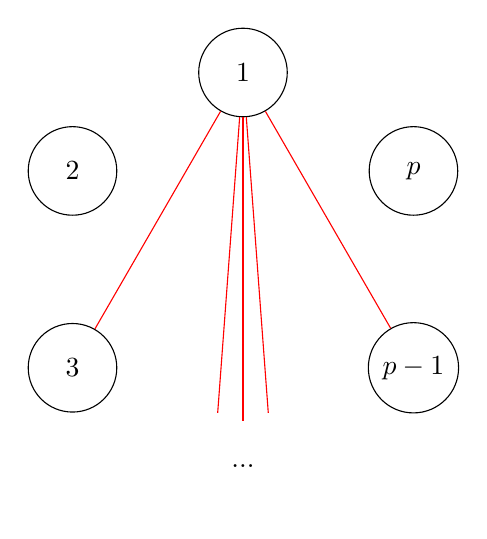
\begin{tikzpicture}[
        point/.style={circle,draw,minimum size=#1},
        point/.default=0pt
    ]
        % \coordinate[label = above:1] (1) at (90:3);
        % \node at (1)[circle,fill,inner sep=2pt]{};

        \node[point=3.2em] (1) at (90:2.5) {1};
        \node[point=3.2em] (2) at (150:2.5) {2};
        \node[point=3.2em] (3) at (210:2.5) {3};
        \node[point=3.2em, draw=none] (dots) at (270:2.5) {...};
        \node[point=3.2em] (pm1) at (330:2.5) {$p-1$};
        \node[point=3.2em] (p) at (30:2.5) {$p$};


        \centerarc[](0,0)(105:135:2.5)
        \centerarc[](0,0)(165:195:2.5)
        \centerarc[](0,0)(225:255:2.5)
        \centerarc[](0,0)(285:314.5:2.5)
        \centerarc[](0,0)(345.5:375:2.5)
        \centerarc[](0,0)(45:75:2.5)

        \draw (1) edge[red] (3);
        \draw (1) edge[red] (dots);
        \draw (1) edge[red] (pm1);
        \draw (1) edge[red] (260:1.85);
        \draw (1) edge[red] (280:1.85);
        
    \end{tikzpicture}
    \caption{The graph $\G = ([p], E)$ formed from the black edges in the above figure is the cycle of length $p$. If $E^+$ is formed by adding the red edges in the figure to $E$, $\G^+ = ([p], E^+)$ forms a chordal cover of $\G$.}
    \label{fig-pcycle}
\end{figure}

\begin{example} \label{ex-pcycle}
    Let $\G = ([p], E)$ be a chordless cycle of length $p \geq 4$, $E = \eset{ (1, 2), (2, 3), \ldots, (p, 1)}$. Then, the maximal clique size of $\G$ is $q(\G) = 2$. We can form a chordal cover $\G^+ = ([p], \G^+)$ that attains the minimum $q(\G^+) = 3$ by connecting an arbitrary node $a$ to all other nodes of $\G$ that are not already a neighbour of $a$. That is, we define the set of edges of $\G^+$ as $E^+ = E \cup \eset{ (a, i) : i \in [p] \setminus \eset{a}}$. This chordal covering is depicted in Figure \ref{fig-pcycle}, with $a = 1$. Hence, for a chordless cycle $\G$ of size $p$,
    \begin{equation*}
        2 \leq \t{mlt}(\G) \leq 3.
    \end{equation*}
    The exact conditions under which the maximum likelihood estimator in a chordless cycle exists for $n = 2$ are studied in Buhl \cite[Section 4]{Buhl1993OnTE}.
\end{example}


Now that we have presented some of the conditions under which one can almost surely find a positive definite completion to the $\G$-partial correlation matrix $S^\G$, we turn ourselves to the question of finding an algorithm capable of computing the maximum likelihood estimator $\hat\Sigma$ of $\Sigma$. As discussed earlier, the completely specified principal submatrices of $S^\G$ are the submatrices corresponding to the cliques of $\G$. Hence, finding a positive definite completion of $\S^\G$ is equivalent to finding the matrix $\hat\Sigma$ satisfying for all $C \in \c(C)(\G)$,
\begin{equation} \label{eq-clique-constraint}
    \hat\Sigma_C = S_C.
\end{equation}
This equation naturally suggests an iterative algorithm successively adjusting parts of the covariance matrix to satisfy (\ref{eq-clique-constraint}) while keeping the running matrix positive definite. This procedure, called \textit{iterative proportional scaling}, was studied by Speed and Kiiveri \cite{speed1986gaussian}, among with other algorithms for solving the maximum equation problem in a Gaussian graphical model. 

Next, we present a development of the algorithm in a Gaussian graphical model with graph $\G$ given a sample covariance matrix $C$ computed from a sample of size $n > \t{mlt}(\G)$. Let $\Omega \in \S^p_{\succ 0}$ be a positive definite matrix and let $C \in \c{C}(\G)$ be a clique of $\G$. We define the \textit{$C$-marginal adjustment} operato $T_C$ given by
\begin{equation} \label{eq-tc-1}
    T_C \Omega = \Omega + \begin{pmatrix}
        (S_C)^{-1} - (\Sigma_C)^{-1} & 0\\
        0 & 0 
        \end{pmatrix},
\end{equation}
where the variable $\Sigma$ denotes the inverse of $\Omega$ and, for simplicity of notation, the top-left block of matrices writen out explicitly corresponds to the current clique $C$. We now show that the operator $T_C$ satisfies the following useful properties.


% \begin{lemma} \label{lem-sym-psd}
%     Let $\Sigma \in \S^p$ be a symmetric block diagonal matrix decomposing as
%     \begin{equation*}
%         \Sigma = \begin{pmatrix}
%             A & B\\
%             B^\top & C
%         \end{pmatrix}.
%     \end{equation*}
%     Then, $\Sigma \in \S^p_{\succ 0}$ if and only if both $E = A - BC^{-1}$ and $C$ are positive definite.
% \end{lemma}

% \begin{proof}
%     See 
% \end{proof}

\begin{proposition}
    Let $\G = ([p], E)$ and $S$ be an empirical covariance matrix constructed from a sample of size $n > \t{mlt}{\G}$ from the Gaussian graphical model associated to $\G$. Then, the operator $T_C$ satisfies the following properties.
    \begin{enumerate}[i.]
        \item $T_C$ is well defined;
        \item $T_C$ adjusts the $C$-marginal of $\Omega$. That is, $(T_C \Omega)^{-1}$ satisfies (\ref{eq-clique-constraint}) for the clique $C$;
        \item If $\Omega \in \S^p_{\succ 0}$, then $T_C \Omega \in \S^p_{\succ 0}$;
        \item If $\Omega \in \S(\G)$, then $T_C \Omega \in \S(\G)$.
    \end{enumerate}    
\end{proposition}
\begin{proof}
    (i) By assumption on the sample size $n$, all matrices and submatrices involved in $T_C$ are positive definite and can be inverted.
    \newline
    (ii) As seen earlier, the inverse of $\Sigma_C$ can be expressed in terms of $\Omega$ by using the Schur completement
    \begin{equation*}
        (\Sigma_C)^{-1} = \Omega_C - \Omega_{C, C^c}(\Omega_{C^c})^{-1}\Omega_{C^c, C},
    \end{equation*}
    where the complement $C^c$ is taken in $[p]$, that is, $C^c = [p] \setminus C$. Replacing this in the definition of $T_C$ gives
    \begin{equation} \label{eq-tc-2}
        T_C \Omega = \begin{pmatrix}
            (S_C)^{-1} + \Omega_{C, C^c}(\Omega_{C^c})^{-1}\Omega_{C^c, C} & \Omega_{C, C^c}\\
            \Omega_{C^c, C} & \Omega_{C^c, C^c}
            \end{pmatrix}.
    \end{equation}
    We can now use the Schur complement to compute the $C$-marginal of $\Omega$,
    \begin{align*}
        \left[(T_C \Omega)^{-1}\right]_C 
        &= \left[ (S_C)^{-1} + \Omega_{C, C^c}(\Omega_{C^c})^{-1}\Omega_{C^c, C} - \Omega_{C, C^c}(\Omega_{C^c})^{-1}\Omega_{C^c, C} \right]^{-1}\\
        &= \left[ (S_C)^{-1}\right]^{-1} = S_C.
    \end{align*}
    (iii) In \cite[Proposition B.1]{lauritzen1996}, Lauritzen gives a sufficient condition for a symmetric diagonal to be positive definite. Applying this lemma, we have that $T_C \Omega$ is positive definite if and only if both $(T_C \Omega)_C$ and $E = (T_C \Omega)_C - (T_C \Omega)_{C, C^c}((T_C \Omega)_{C^c})^{-1}(T_C \Omega)_{C^c,C}$ are positive definite. As seen in (ii), $(T_C \Omega)_C = S_C$ is by assumption positive definite. As for the Schur complement
    \begin{align*}
        E &= (T_C \Omega)_C - (T_C \Omega)_{C, C^c}((T_C \Omega)_{C^c})^{-1}(T_C \Omega)_{C^c,C}\\
        &= (S_C)^{-1} + \Omega_{C, C^c}(\Omega_{C^c})^{-1}\Omega_{C^c, C} - \Omega_{C, C^c}(\Omega_{C^c})^{-1}\Omega_{C^c,C}\\
        &= (S_C)^{-1},
    \end{align*}
    is by the same assumption positive definite. Hence $T_C \Omega$ is positive definite.
    \newline
    (iv) Let $E$ be the set of edges of $\G$ and $e = \eset{i, j} \notin E$ be a missing edge in $\G$. Since $C$ is a clique of $\G$, we have that $|C \cap \eset{i, j}| \leq 1$ and the entry of the matrix $T_C \Omega$ corresponding to the edge $\eset{i, j}$ is in one of the following submatrices: $(T_C \Omega)_{C, C^c}$, $(T_C \Omega)_{C^c}$ or $(T_C \Omega)_{C^c,C}$. Since these submatrices are left invariant under $T_C$, we have that $(T_C \Omega)_{ij} = \Omega_{ij} = 0$, thus $T_C \Omega \in \S(\G)$.
\end{proof}

Given these properties, we can naturally define an algorithm by cycling through the cliques $C \in \c{C}(\G)$ of $\G$, successively adjusting each $C$-marginal by applying the adjustement operator $T_C$, and repeating until convergence. This algorithm is the iterative proportional scaling algorithm, given in Algorithm \ref{alg:itpropscale}. The question remains of whether this algorithm converges and why. We start by showing that the $C$-marginal adjustement operator computes the solution to a constrained version of (\ref{eq-primal}).

\begin{algorithm}[ht!]
    \caption{Iterative proportional scaling}
    \label{alg:itpropscale}
    \begin{algorithmic}[1]
    \Require{Set of cliques $\c{C}(\G)$, sample covariance matrix $S$, tolerance $\varepsilon$.} 
    \Ensure{Maximum likelihood estimator $\hat\Omega$.}
    
        \State {Let $\Omega^0 = 1_p$}
        \State {Let $\Omega^1 = \Omega^0$}
        \For{\texttt{$C \in \c{C}(\G)$ }}
            \State{Set $\Omega^1 := T_C \Omega^1$ }
        \EndFor
        \If{$\norm{\Omega^1 - \Omega^0} < \varepsilon$}
            \State{Return $\hat\Omega := \Omega^1$}
        \Else
            \State{Set $\Omega^0 := \Omega^1$}
            \State{Go to line 2.}
        \EndIf
    \end{algorithmic}
\end{algorithm}

\begin{lemma} \label{lem-tc-sol-opt}
    Let $\Omega^0 \in \S_{\succ 0}(\G)$. The $C$-marginal adjustement operator $T_C$ computes the solution to problem (\ref{eq-primal}) over the section 
    \begin{equation*}
        \Theta_C(\Omega^0) = \eset{ \Omega \in \S_{\succ 0}(\G) : \Omega_{C^c} = \Omega^0_{C^c} \t{ and } \Omega_{C, C^c} = \Omega^0_{C, C^c} }.
    \end{equation*}
    That is, $T_C \Omega^0$ is the solution to
    \begin{align} \label{eq-sub-optim}
        \begin{split}
            &\underset{\Omega \in \S_{\succ 0}(\G)}{\t{maximize}}\ \  \log |\Omega| - \tr[S\Omega]\\
            &\t{subject to}\ \ \Omega_{C^c} = \Omega^0_{C^c} \t{ and } \Omega_{C, C^c} = \Omega^0_{C, C^c}.
        \end{split}
    \end{align}
\end{lemma}
\begin{proof}
    Using the expression of the determinant of a block matrix in terms of Schur complement, we have that
    \begin{equation*}
        \abs{\Omega} 
        = \abs{\Omega_C - \Omega_{C, C^c}(\Omega_{C^c})^{-1}\Omega_{C^c, C}} \abs{\Omega_{C^c}}.
    \end{equation*}
    Furthermore, using the fact that $\Omega \in \Theta(\Omega^0)$, it follows that
    \begin{align*}
        \log \abs{\Omega}
        &= \log \left\{ \abs{\Omega_C - \Omega^0_{C, C^c}(\Omega^0_{C^c})^{-1}\Omega^0_{C^c, C}} \abs{\Omega^0_{C^c}} \right\}\\
        &= \log \abs{\Omega_C - \Omega^0_{C, C^c}(\Omega^0_{C^c})^{-1}\Omega^0_{C^c, C}} + \log \abs{\Omega^0_{C^c}}\\
        &= \log \abs{\Omega'} + \log \abs{\Omega^0_{C^c}},
    \end{align*}
    where $\Omega' = \Omega_C - \Omega^0_{C, C^c}(\Omega^0_{C^c})^{-1}\Omega^0_{C^c, C}$. Since $\Omega^0_{C^c}$ is constant in the optimization problem (\ref{eq-sub-optim}), it can be ignored and we have $\log \abs{\Omega}$ and $\log \abs{\Omega'}$ are equal up to a constant term. Furthermore, using again the fact that $\Omega \in \Theta_C(\Omega^0)$, we get
    \begin{align*}
        \trB{\Omega S}
        &= \trB{\Omega_C S_C} + \trB{\Omega_{C^c} S_{C^c}} + 2 \trB{\Omega_{C,C^c} S_{C,C^c}} 
        \doteq \trB{\Omega_C S_C} \\
        &= \trB{\Omega'S_C} + \trB{\Omega^0_{C, C^c}(\Omega^0_{C^c})^{-1}\Omega^0_{C^c, C}S_C}
        \doteq  \trB{\Omega'S_C}.
    \end{align*}
    Hence, the optimization problem (\ref{eq-sub-optim}) is equivalent to 
    \begin{equation*}
        \underset{\Omega' \in \S_{\succ 0}^{|C|}}{\t{maximize}}\ \  \log |\Omega'| - \tr[S_C\Omega'].
    \end{equation*}
    Comparing this to the earlier discussions, this problem is equivalent to finding the maximum likelihood estimator of the precision matrix $\Omega'$ of the Gaussian graphical model associated to the graph $\G$ restricted to the nodes in $C$. Since $C$ is a clique, the subgraph is complete and the maximum likelihood estimator is given by $\hat\Omega' = (S_C)^{-1}$. Hence, the solution to (\ref{eq-sub-optim}) is given by $\hat\Omega \in \Theta(\Omega^0)$ where
    \begin{align*}
        \hat\Omega_C
        &= \Omega' + \Omega^0_{C, C^c}(\Omega^0_{C^c})^{-1}\Omega^0_{C^c, C}\\
        &= (S_C)^{-1} + \Omega^0_{C, C^c}(\Omega^0_{C^c})^{-1}\Omega^0_{C^c, C}.
    \end{align*}
    Hence the solution to (\ref{eq-sub-optim}) is $\hat\Omega = T_C \Omega^0$.
\end{proof}

By Lemma \ref{lem-tc-sol-opt}, Algorithm \ref{alg:itpropscale} corresponds to an \textit{iterative partial maximization} algorithm, or block coordinate descent algorithm. Since $T_C$ is a linear transformation, it is continuous. Further, we showed that $T_C$ maps $\S_{\succ 0}(\G)$ onto itself. With these conditions satisfied, Lauritzen \cite[Proposition A.3]{lauritzen1996} proves that the iterative partial maximization algorithm converges and hence, Algorithm \ref{alg:itpropscale} converges to the maximum likelihood estimator $\hat\Omega \in \S_{\succ 0}(\G)$.

\subsection{Hypothesis testing}


We now turn ourselves to applying the approximations developed in Section \note{todo} on the problem of testing two nested Gaussian graphical models. More precisely, let $\G = (\Gamma, E)$ and $\G_0 = (\Gamma, E_0)$ with $E_0 \subset E$, we are interested in developing a test for the problem
\begin{equation} \label{eq-null-general-graph}
    H_0 : \Omega \in \S_{\succ 0}(\G_0)\ \ \t{ vs. }\ \ H_1 : \Omega \in \S_{\succ 0}(\G) \setminus \S_{\succ 0}(\G_0).
\end{equation}
The classical approach for testing this problem is to use the \textit{likelihood ratio test} based on the \textit{likelihood ratio statistic}. Given an observed covariance matrix $S_n$ constructed from a sample of size $n$, the likelihood ratio statistic is given by
\begin{equation*}
    \Lambda(S_n) = -2 \left[\ell(\hat\Omega_{\G_0}(S_n)) - \ell(\hat\Omega_\G(S_n))\right],
\end{equation*}
where $\hat\Omega_{\G_0}$ and $\hat\Omega_\G$ are the functions mapping an observed covariance matrix to the maximum likelihood estimators of the precision matrix under the model $\G_0$ and $\G$. Under regularity conditions and assuming that the $H_0$ is true, the distribution of $\Lambda(S_n)$ converges to a $\chi^2_d$ distribution with $d = |E| - |E_0|$. A hypothesis test in final sample can then be constructed by using the $\chi^2_d$ approximation to the distribution of $\Lambda(S_n)$.

In Eriksen \cite{eriksen1996tests}, the author gives a simple example for which we can demonstrate how this approximation fails when the sample size $n$ is not large enough. Consider two graphs $\G$ and $\G_0$ with $p = 4$ nodes such that $\G_0$ is a cycle and $\G$ is a chordal cover of $\G$. We are then interested in the following hypothesis test in Figure \ref{fig-test-cycle-vs-diamond}. Eriksen proposes an alternative test statistic for testing this class of problem which, in this examples is
\begin{equation} \label{eq-q-stat}
    Q(S_n) = \expf{-\Lambda(S_n) / n},
\end{equation}
which asymptotically follows a beta distribution $B((n - 3)/2, 1/2)$.



As we have seen in the previous section, the maximum likelihood estimator exists under both $H_0$ and $H_1$ almost surely if $n \geq 3$. We can then empirically evaluate the $\chi_2^d$ approximation to the distribution of $\Lambda(S_n)$ and $B((n - 3)/2, 1/2)$ approximation to the distribution of $Q(S_n)$ by sampling the statistics under the null hypothesis of a chordless cycle. For a given sample size $n \in \N$, we sample $N = 10000$ values $\lambda_1, \ldots, \lambda_N$ of the statistic $\Lambda(S_n)$ under the null hypothesis. With this sample, we can construct the empirical cumulative distribution function $\hat F_\Lambda$ which approximates the true cumulative distribution function of $\Lambda(S_n)$, as well as the sorted empirical probabilities $\hat p_{i} = \hat F_\Lambda(\lambda_{(i)})$. The empirical probabilities $\hat p_{i}$ can then be compared to the probabilities $\tilde p_i = F(\lambda_{(i)})$ where $F$ corresponds to the cumulative distribution function of either the $\chi^2_1$ approximation of $\Lambda(S_n)$ or the $B((n - 3)/2, 1/2)$ approximation of $Q(S_n) = \expf{-\Lambda(S_n) / n}$. Figure \ref{fig-diamond-vs-square-small}, displays this comparison. As we can see in the upper pane of Figure \ref{fig-diamond-vs-square-small}, the $\chi^2_1$ approximation is a poor approximation to the distribution of $\Lambda(S_n)$ while the $B((n - 3)/2, 1/2)$ approximation to the distribution of $Q(S_n)$ is accurate even for small sample sizes. Since we are interested in constructing a hypothesis test based on these approximation, the small probability region is of particular interest. In the lower pane of Figure \ref{fig-diamond-vs-square-small}, we see that the $\chi^2_1$ approximation is particularly bad for $n=5$ where a test at level $\alpha=0.05$ based on the $\chi^2_1$ approximation would have a true size of $0.1$.
\begin{figure}[tbp!]
    \begin{minipage}[c]{.45\linewidth}
        \centering
        $\ \ \ \ \ \ \ \ \ \ \ \ \ H_0$
        \newline
        \newline
        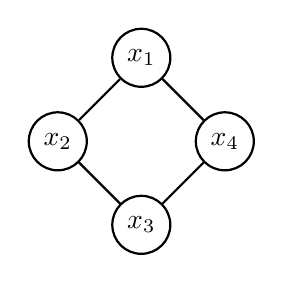
\begin{tikzpicture}[node distance={15mm}, thick, main/.style = {draw, circle}] 
            \node[main] (1) {$x_1$}; 
            \node[main] (2) [below left of=1] {$x_2$};
            \node[main] (3) [below right of=2] {$x_3$}; 
            \node[main] (4) [above right of=3] {$x_4$};
            \draw (1) -- (2);
            \draw (2) -- (3);
            \draw (4) -- (3);
            \draw (1) -- (4);
        \end{tikzpicture}
    \end{minipage}
    \begin{minipage}[c]{.1\linewidth}
        \centering
        $ $
        \newline\newline
        vs.
    \end{minipage}
    \begin{minipage}[c]{.45\linewidth}
        \centering
        $\ \ \ \ \ \ \ \ \ \ \ \ \ H_1$
        \newline
        \newline
        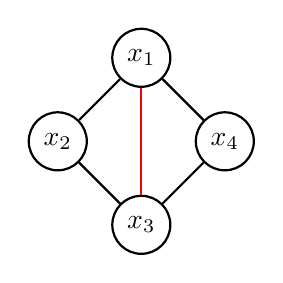
\begin{tikzpicture}[node distance={15mm}, thick, main/.style = {draw, circle}] 
            \node[main] (1) {$x_1$}; 
            \node[main] (2) [below left of=1] {$x_2$};
            \node[main] (3) [below right of=2] {$x_3$}; 
            \node[main] (4) [above right of=3] {$x_4$};
            \draw (1) -- (2);
            \draw (2) -- (3);
            \draw (4) -- (3);
            \draw (1) -- (4);
            \draw (1) edge[red] (3);
        \end{tikzpicture}
    \end{minipage}
    \caption{Simple hypothesis test proposed by Eriksen \cite{eriksen1996tests} for which the $\chi^2_1$ approximation to the likelihood ratio statistic fails.}
    \label{fig-test-cycle-vs-diamond}
\end{figure}
\begin{figure}[!tbp]
    \centering
    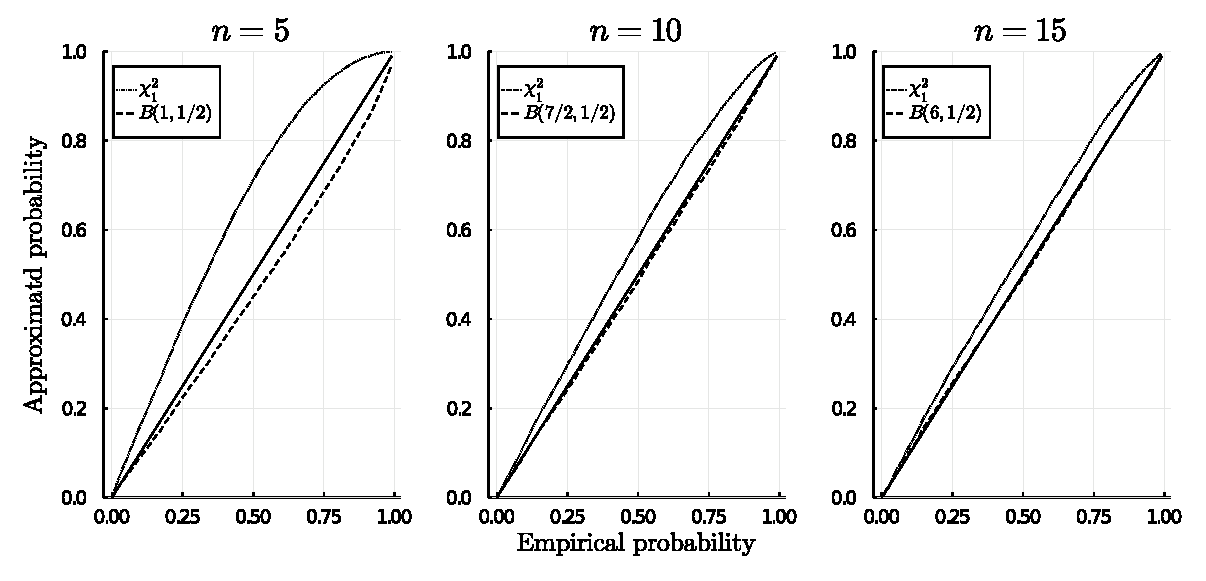
\includegraphics[width=16cm]{diamond_vs_square_0_1}
    \newline
    \newline
    \newline
    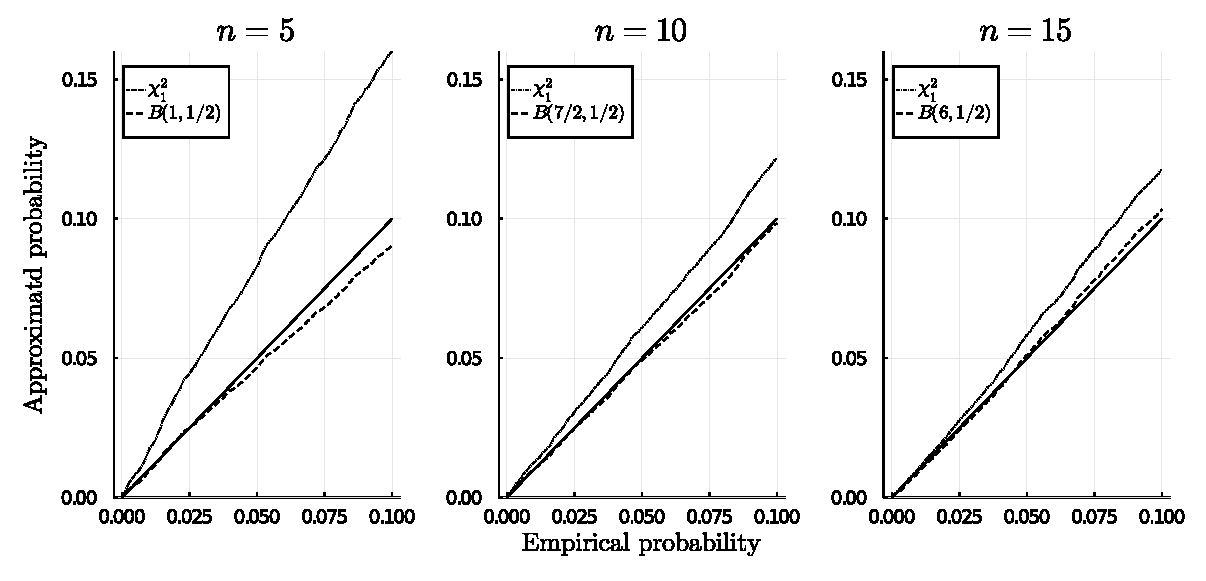
\includegraphics[width=16cm]{diamond_vs_square_0_01}
    \caption{Comparison of the $\chi^2_1$ approximation of the $\Lambda(S_n)$ statistic and Beta approximation of the $Q(S_n)$ statitistic from Eriksen \cite{eriksen1996tests} for testing the null hypothesis of a chordless cycle given a sample of $n = 5, 10, 15$ observations. As seen in the upper pane, the $\chi^2_1$ approximation poorly estimates the distribution of the $\Lambda(S_n)$ statistic for small and moderate sample sizes, while the $B((n - 3)/2, 1/2)$ approximation to the distribution of $Q(S_n)$ is accurate even for small sample sizes. This is particularly strong when focusing on small probability regions as we show in the lower pane where the difference of probability can be of approximately 50\%.}
    \label{fig-diamond-vs-square-small}
\end{figure}


While the $B((n - 3)/2, 1/2)$ approximation seems accurate, it is not yet clear where it comes from and why it works. In the rest of this section based on Eriksen \cite{eriksen1996tests}, we present the construction of this statistic as well as proof of convergence. In the following lemma, we apply the $p^*$ approximation to construct an accurate estimation to the density of the sufficient statistic $S$.

\begin{lemma} \label{lem-pstar-covariance}
    Let $\G$ be a graph, $\Omega \in \S_{\succ 0}(\G)$ and $S$ be a sample covariance matrix computes from a sample of size $n$ of the Gaussian graphical model associated to $\G$ with precision matrix $\Omega$. Then, the density $p(S; \Omega)$ of $S$ satisfies
    \begin{equation*}
        p(S; \Omega) = c \frac{|\Omega|^{n/2}}{|\hat\Omega_\G(S)|^{n/2}} |j_\G(\hat\Omega_\G(S)) |^{-1/2} \expfc{-\frac{n}{2} \trB{\Omega S}} (1 + O(n^{-3/2})),
    \end{equation*}
    where $c$ is a normalization constant, $\hat\Omega_\G(S)$ is the maximum likelihood of $\Omega$ assuming the graph $\G$ and given the data $S$, and $j_G$ is the observed information matrix given by
    \begin{equation} \label{eq-obs-info}
        j_\G(\Omega)_{a b} = \trB{\Omega^{-1} H_a \Omega^{-1} H_b} \t{ for all } a, b  \in E.
    \end{equation}
\end{lemma}

\begin{proof}
    Since $XX^\top$ is sufficient in the Gaussian graphical model, $S$ corresponds to the sample average of the sufficient statistic. Applying the $p^*$ approximation to $S$ as done in Section \note{todo}, we have that the density of $S$ satisfies
    \begin{equation*}
        p(S; \Omega) = c |j_\G(\hat\Omega_\G(S))|^{-1/2} \expfc{\ell(\Omega; S) - \ell(\hat\Omega_\G(S); S)} (1 + O(n^{-3/2})).
    \end{equation*}
    Replacing the log-likelihood of the Gaussian graphical model in the above equation, we get
    \begin{align*}
        p(S; \Omega) 
        &\propto |j_\G(\hat\Omega_\G(S))|^{-1/2} \expfc{\ell(\Omega; S) - \ell(\hat\Omega_\G(S); S)} (1 + O(n^{-3/2})) \\
        &\propto |j_\G(\hat\Omega_\G(S))|^{-1/2} 
        \frac{|\Omega|^{n/2}}{|\hat\Omega_\G(S)|^{n/2}}
        \expfc{-\frac{n}{2}\left(\trB{\Omega S} - \trB{\hat\Omega_\G(S) S}\right)} (1 + O(n^{-3/2}))\\
        &\propto |j_\G(\hat\Omega_\G(S))|^{-1/2} 
        \frac{|\Omega|^{n/2}}{|\hat\Omega_\G(S)|^{n/2}}
        \expfc{-\frac{n}{2}\trB{\Omega S}} (1 + O(n^{-3/2}))
    \end{align*}
    where we use that $\hat\Omega_\G(S) S = 1_p$ and hence $\trB{\hat\Omega_\G(S) S} = p$ is constant. The formula for the observed infomation matrix can be easily verified by taking the appropriate derivatives of the log-likelihood.
\end{proof}

Before applying the result of Lemma \ref{lem-pstar-covariance} to the general problem of subgraph testing, we start with studying a special case. Consider a Gaussian graphical model with graph $\G = ([p], E)$ and the sub-model constructed by remove an edge $a \in E$ from $\G$. The sub-model is then the Gaussian graphical model associated to the graph $\G_0 = ([p], E_0)$ where $E_0 = E \setminus \eset{e_0}$. Without loss of generality, we assume $e_0 = \eset{1,2}$. The test statistic given in (\ref{eq-q-stat}) is then
\begin{align*}
    Q(S_n) 
    &= \expf{-\Lambda(S_n) / n}  \\
    &= \expf{2 \left[\ell(\hat\Omega_{\G_0}(S_n)) - \ell(\hat\Omega_\G(S_n))\right] / n} \\
    &= \expf{
        (\log |\hat\Omega_{\G_0}(S_n)| - \tr[S_n\hat\Omega_{\G_0}(S_n)])
        -    
        (\log |\hat\Omega_\G(S_n)| - \tr[S_n\hat\Omega_\G(S_n)])} \\
    &= \frac{|\hat\Omega_{\G_0}(S_n)|}{|\hat\Omega_{\G}(S_n)|},
\end{align*}
where we have used that $\tr[S_n\hat\Omega_{\G_0}(S_n)] = p$ is constant given any assumed graph. In the following theorem, we show that the $Q(S_n)$ statistic asymptotically follows a beta distribution with known parameters.

\begin{theorem} \label{thm-one-edge-less}
    Let $\G = ([p], E)$ be a graph with subgraph $\G_0 = ([p], E_0)$ with $E \setminus E_0 = \eset{e_0}$. Let $S$ be a sample covariance matrix computed from a sample of size $n$ of the Gaussian graphical model associated to $\G_0$ with precision matrix $\Omega_0 \in \S_{\succ 0}(\G_0)$. Then, the distribution of $Q(S_n)$ conditioned on observing $S_n$ is asymptotically
    \begin{equation}
        Q(S_n) \sim B\left(\frac{n - f(e_0) - 1}{2}, \frac{1}{2} \right)\ \ \ \ \t{ as } n \rightarrow \infty,
    \end{equation}
    where $f(\eset{i, j}) = |\t{bd}(i) \cap \t{bd}(j)|$.
\end{theorem}
\begin{proof}
    We can then construct approximations to the densities $p(S^{\G_0}; \Omega_0)$ and $p(S^{\G}; \Omega_0)$ by applying Lemma \ref{lem-pstar-covariance} in the Gaussian graphical models associated to $\G$ and $\G_0$ to get
    \begin{equation*}
        p(S^{\G_0}; \Omega_0) = c \frac{|\Omega_0|^{n/2}}{|\hat\Omega_{\G_0}(S^{\G_0})|^{n/2}} |j_{\G_0}(\hat\Omega_{\G_0}(S^{\G_0})) |^{-1/2} \expfc{-\frac{n}{2} \trB{\Omega_0 S^{\G_0}}} (1 + O(n^{-3/2}))
    \end{equation*}
    and
    \begin{equation*}
        p(S^\G; \Omega_0) = c \frac{|\Omega_0|^{n/2}}{|\hat\Omega_\G(S^\G)|^{n/2}} |j_\G(\hat\Omega_\G(S^\G)) |^{-1/2} \expfc{-\frac{n}{2} \trB{\Omega_0 S^\G}} (1 + O(n^{-3/2})).
    \end{equation*}
    Combining these results together allows us to approximate the density of $S_e$ conditioned on $S^{\G_0}$
    \begin{align*}
        p(S_{e_0}| S^{\G_0}; \Omega_0)
        &= \frac{p(S_{e_0}, S^{\G_0}; \Omega_0)}{p(S^{\G_0}; \Omega_0)} = \frac{p(S^{\G}; \Omega_0)}{p(S^{\G_0}; \Omega_0)}\\
        & \doteq \tilde c 
        \frac
            {|\Omega_0|^{n/2}|\hat\Omega_{\G_0}(S^{\G_0})|^{-n/2} |j_{\G_0}(\hat\Omega_{\G_0}(S^{\G_0})) |^{-1/2} \expfc{-\frac{n}{2} \trB{\Omega_0 S^{\G_0}}}}
            {|\Omega_0|^{n/2}|\hat\Omega_\G(S^\G)|^{-n/2} |j_\G(\hat\Omega_\G(S^\G)) |^{-1/2} \expfc{-\frac{n}{2} \trB{\Omega_0 S^\G}}}\\
        &= \tilde c 
        \frac
            {|\hat\Omega_\G(S^\G)|^{n/2} |j_\G(\hat\Omega_\G(S^\G)) |^{1/2}}    
            {|\hat\Omega_{\G_0}(S^{\G_0})|^{n/2} |j_{\G_0}(\hat\Omega_{\G_0}(S^{\G_0})) |^{1/2}}\\
        &= q^{n/2} \frac{|j_\G(\hat\Omega_\G(S^\G)) |^{1/2}}    {|j_{\G_0}(\hat\Omega_{\G_0}(S^{\G_0})) |^{1/2}}.
    \end{align*}
    where we used in the last step that $\Omega_0 S^\G = \Omega_0 S^{\G_0}$ which leads to the exponential terms canceling out. Since $w \xrightarrow{d} \chi^2_1$ is asymptotically ancillary, and $q = \expfc{-\frac{1}{2} w}$, $q$ is also asymptotically ancillary. Since $S^{\G_0}$ is a complete sufficient statistic assuming $\G_0$, $S^{\G_0}$ and $q$ are asymptotically independent by Basu's Theorem \cite{10.2307/25048259}. This means that asymptotically $p(S_{e_0}; \Omega_0) = p(S_{e_0} | S^{\G_0}; \Omega_0)$ for any $S^{\G_0}$ and we can chose $S^{\G_0}$ freely in the previous equation. Taking $S^{\G_0} = 1_p$ gives
    \begin{equation*}
        S^\G = 1_p + S_{e_0} H_{e_0} = \begin{pmatrix}
            1   & S_{e_0} & \\
            S_{e_0} & 1 & \\
                &   & 1_{p-2}
        \end{pmatrix}.
    \end{equation*}
    Since $S^{\G_0}$ and $S^\G$ are positive definite, they are their own positive definite completion and we have $|\hat\Omega_\G(S^\G)| = |S^\G|^{-1} = (1 - S_{e_0}^2)^{-1}$ and $|\hat\Omega_{\G_0}(S^{\G_0})| = |S^{\G_0}|^{-1} = 1$, giving $q = 1 - S_{e_0}^2$. A change of variable from $S_e$ to $q$ has Jacobian $(1 - q)^{-1/2}$ and the density of $q$ can be given by
    \begin{equation} \label{eq-proof-almost-done}
        p(q) \doteq \hat c q^{n/2} |j_{\G}(\hat\Omega_{\G}(S^{\G})) |^{-1/2} (1 - q)^{-1/2},
    \end{equation}
    for some normalizing constant $\hat c$.

    We now bring our attention to computing the determinant of the observed information matrix given in (\ref{eq-obs-info}) with $\Omega^{-1} = 1_p + S_e H_e$. Let $a, b \in E$, we start by noting that for any $S \in \S(\G)$ and $i, j \in [p]$
    \begin{equation*}
        (SH_a)_{ij} = \begin{cases}
            & S_{i \bar j}\ \ \t{ if } j \in a\\
            &0\ \ \ \ \  \t{otherwise}
        \end{cases}
        \ \ \ \t{ and }\ \ \ \ \ 
        (SH_b)_{ji} = \begin{cases}
            & S_{j \bar i}\ \ \t{ if } i \in b\\
            &0\ \ \ \ \  \t{otherwise}
        \end{cases},
    \end{equation*}
    where $\bar j \in a$ and $\bar i \in b$ are such that $\eset{j} \cup \eset{\bar j} = a$ and $\eset{i} \cup \eset{\bar i} = b$. Using this in the expression of $j_\G(S)_{ab}$, we get
    \begin{equation} \label{eq-tr-sum}
        \trB{SH_aSH_b} = \sum_{i=1, j=1}^p (SH_a)_{ij}(SH_b)_{ji} = \sum_{(i, j) \in a \times b} S_{i \bar j} S_{j \bar i} = \sum_{e \in a \times b} S_e S_{\bar e},
    \end{equation}
    where the last equality only involves re-indexing and re-ordering the sum. We now inspect the different $a, b$ for which the summand $S_eS_{\bar e}$ is non-zero. Setting $s = S_{e_0}$, we have $S = 1_p + s H_{e_0}$ and hence for any $e \in E$
    \begin{equation*}
        S_e = \begin{cases}
            &1\ \ \t{ if } e = \eset{ i } \t{ for } i \in [p]\\
            &s\ \ \t{ if } e = e_0\\
            &0\ \ \t{ otherwise}.
        \end{cases}
    \end{equation*}
    Thus, the summands $S_e S_{\bar e}$ of (\ref{eq-tr-sum}) are non-zero if and only if both $e$ and $\bar e$ are either $\eset{i}$ for some $i \in [p]$ or equal to $e_0$. Without loss of generality, we will assume that $e_0 = \eset{1, 2}$. This leaves us with the following cases. 

    Case 1. $e = \bar e = \eset{1, 2}$. This can only happen if $a = \eset{1}$ and $b = \eset{2}$, in which case
    \begin{equation*}
        j_\G(S)_{\eset{1} \eset{2}} = \sum_{e \in \eset{1} \times \eset{2}} S_e S_{\bar e} = S_{\eset{1, 2}}S_{\eset{1, 2}} = s^2.
    \end{equation*}

    Case 2. $e = \eset{1, 2}$ and $\bar e = \eset{i, j}$ with $i \neq j$ (or the opposite). Then we must have $a = \eset{1, i}$ and $b = \eset{2, j}$ and
    \begin{equation*}
        j_\G(S)_{\eset{1, i} \eset{2, j}} = S_{1 2}S_{i j} + S_{1 j} S_{i 2} + S_{i 2} S_{1 j} + S_{i j} S_{1 2} = 0,
    \end{equation*}
    since we assumed that $S = 1_p + s H_{e_0}$.

    Case 3. $e = \eset{1, 2}$ and $\bar e = \eset{i}$ (or the opposite). This is the case when $a = \eset{1, i}$ and $b = \eset{2, i}$ and we get
    \begin{equation*}
        j_\G(S)_{\eset{1, i} \eset{2, i}} = 
        S_{1 2}S_{i i} + S_{1 i} S_{i 2} + S_{i 2} S_{1 i} + S_{i i} S_{1 2} = 2 s,
    \end{equation*}
    since $S_{i i} = 1$, $S_{1, 2} = s$ and $S_{i 1} = S_{i 2} = 0$. Note that since the matrix $j_\G$ is indexed by edges in $\G$, the cases $a = \eset{1, i}$ and $b = \eset{2, i}$ are only relevant if $a, b \in E$ and so this case only for $i \in C = \t{bd}(1) \cap \t{bd}(2)$.

    Case 4. $e = \eset{i}$ and $\bar e = \eset{j}$. This only happens is $a = b = \eset{i, j}$, which, again using that $a, b \in E$ and $S = 1_p + sH_{e_0}$ gives
    \begin{equation*}
        j_\G(S)_{\eset{i, j} \eset{i, j}} = \begin{cases}
            &S_\eset{i, i}S_\eset{i, i} = 1\ \ \ \ \ \ \ \ \ \ \ \ \ \ \ \ \ \ \ \ \ \ \ \ \ \ \ \  \t{ if } i = j\\
            &2S_\eset{1 1}S_\eset{2 2} + 2S_\eset{1 2}S_\eset{1 2} = 2 + 2s^2\  \t{ if } \eset{i, j} = \eset{1, 2}\\
            &2S_\eset{i,i} + 2S_\eset{i, j} = 2\ \ \ \ \ \ \ \ \ \ \ \ \ \ \ \ \ \ \ \ \  \t{ otherwise.}
        \end{cases}
    \end{equation*}
    This shows that $j_\G(S)$ is a block diagonal matrix with blocks each equal to one of the following matrices
    \begin{equation*}
        A = \bordermatrix{~ & \eset{1} & \eset{2} & \eset{1, 2} \cr
            \eset{1} & 1 & s^2 & 2s \cr
            \eset{2} & s^2 & 1 & 2s \cr
            \eset{1, 2} & 2s & 2s & 2 + 2s^2 \cr
        }
        \ \ \ \ \ \ \ \ \ 
        B_i = \bordermatrix{~ & \eset{1, i} & \eset{2, i} \cr
            \eset{1, i} & 2 & 2s \cr
            \eset{2, i} & 2s & 2 \cr
        }, i \in C.
    \end{equation*}
    Since $|A| = 2 (1-s^2)^3$ and $|B_i| = 4(1-s^2)$ for $i \in C$, we have that the determinant of the observed information $\abs{j_\G(1_p + sH_{e_0})} \propto (1-s^2)^{3 + |C|} = (1 - S_{e_0}^2)^{3 + f(e_0)} = q^{3 + f(e_0)}$. Replacing this in (\ref{eq-proof-almost-done}) gives
    \begin{align*}
        p(q) 
        &\doteq \hat c q^{n/2} |j_{\G}(\hat\Omega_{\G}(S^{\G})) |^{-1/2} (1 - q)^{-1/2}\\
        &\propto q^{n/2} q^{-(3 + f(e_0))/2} (1 - q)^{-1/2} \\
        &= q^{(n - f(e_0) - 3)/2}(1-q)^{-1/2}.
    \end{align*}
    Since the density of a $B(\alpha, \beta)$ distribution is proportional to $q^{\alpha-1}(1-q)^{\beta-1}$ we have that $q$ asymptotically follows a $B((n - f(e_0) - 1)/2, 1/2)$ distribution.
\end{proof}

This construction can be generalized to the case where $d = |E \setminus E_0| > 1$. Let $E_- = E \setminus E_0 = \eset{e_0, \ldots, e_{d-1}}$, we define for $i = 1, \ldots, d-1$ the subgraphs $\G_i = ([p], E_i)$ with $E_i = E_{i-1} \cup \eset{e_i}$. Then, the $Q(S_n)$ statitistic can be decomposed as 
\begin{align*}
    Q(S_n) 
    &= \frac{|\hat\Omega_{\G_0}(S_n)|}{|\hat\Omega_{\G}(S_n)|}
    = \frac{|\hat\Omega_{\G_0}(S_n)|}{|\hat\Omega_{\G_{d-1}}(S_n)|} \\
    &= \frac{|\hat\Omega_{\G_0}(S_n)|}{|\hat\Omega_{\G_1}(S_n)|}
    \frac{|\hat\Omega_{\G_1}(S_n)|}{|\hat\Omega_{\G_2}(S_n)|}
    \ldots
    \frac{|\hat\Omega_{\G_{d-2}}(S_n)|}{|\hat\Omega_{\G_{d-1}}(S_n)|}
    =: Q_{0,1}(S_n)Q_{1,2}(S_n) \ldots Q_{d-2, d-1}(S_n),
\end{align*}
where $Q_{i, i+1}(S_n)$ corresponds to the test statistic for testing the submodel $\G_i$ in $\G_{i+1}$. Applying Theorem \ref{thm-one-edge-less} to each $Q_{i, i+1}(S_n)$ gives that, asymptotically
\begin{equation*}
    Q_{i, i+1}(S_n) \sim B\left(\frac{n - f(e_i) - 1}{2}, \frac{1}{2} \right) =: B(\alpha_i, 1/2)
\end{equation*}
where $f(e_i) = |\t{bd}(j) \cap \t{bd}(k)|$ for $e_i = \eset{j, k}$ is to be evaluated in the graph $\G_{i+1}$. Hence $Q(S_n)$ is asymptotically distributed as the product of independent $B(\alpha_i, 1/2)$ random variables.


\subsection{Simulation studies}

We now compare different properties of the likelihood ratio test and Eriksen test described in \ref{sec-hyp-test}. We are interested in evaluating the size and power of the tests resulting from these two asymptotic approximations. The \textit{size} of a test is its probability of rejecting the null hypothesis when it is true, also called \textit{type I error}. The \textit{power} of a test is its probability to reject the null hypothesis when it is false. One is interested in tests maximizing power while keeping the probability of doing a type I error under a pre-defined level $\alpha$. In other words, a good test maximizes the probability of discovering true phenomena while maintaining a low probability of making a false discovery. 

We now present experiments aiming at exploring the size and power of the statistical tests constructed based on the $\chi^2_d$ approximation to the distribution of the $\Lambda(S_n)$ statistic and the product of Betas approximation to the distribution of the $Q(S_n)$ statistic. In particular, we are interested in evaluating how the different tests behave when the sample size is kept fix and the number of parameters increases.

Note that the Eriksen approximation to the distribution of $Q(S_n)$ is based on the product of independent Beta distributed random variables $\prod_{i=1}^d B_i$, which does not admit a closed form. Instead, we construct an estimator to the distribution of $\prod_{i=1}^d B_i$ by sampling $100\ 000$ observations of the vector $(B_1, \ldots, B_d)$ and use the product of the sample to construct the empirical estimator to the distribution function.

In the first setup, we consider a sequence of problems in which the number of nodes in a graph $\G$ grows while the number of edges removed to form $\G_0$ is kept fix. In particular, we  consider the complete graph $\G = ([p], E)$ with $E = \eset{\eset{i, j} : i, j \in [p], i \neq j}$ and the subgraph $\G_0 = ([p], E_0)$ with $E_0 = E \setminus \eset{\eset{1, 3}, \eset{2, 4}}$. As shown in Figure \ref{fig-graph-exp-1}, the subgraph $\G_0$ can be decomposed into the cycle $\eset{1, 2, 3, 4}$ and the clique $C_p = [p] \setminus \eset{1,2,3,4}$ formed with the rest of the nodes, such that each node of the cycle forms a clique when added to $C$. 
% In $\G_0$, the largest clique is $C \cup \eset{i}$ for $i \in \eset{1, 2, 3, 4}$ which has a size of $p - 3$. The minimal chordal cover of $\G_0$ can be constructed by adding back the edge $\eset{1, 3}$ or $\eset{2, 4}$ to break to cycle. If we consider the chordal cover constructed by additing the edge $e = \eset{1, 2}$, the maximal clique is $C \cup \eset{1, 2, 4}$ which contains $p - 1$ nodes. Hence, from (\ref{eq-mlt-bounds}), the maximum likelihood threshold $\G_0$ satisfies
% \begin{equation*}
%     p - 3 \leq \t{mlt}(\G_0) \leq p - 2,
% \end{equation*}
% and the maximum likelihood estimator of $\Omega$ under $\G_0$ exists almost surely if $n \geq p - 2$.

In this setup, the quantities of interest are the entries of the precision matrix corresponding to the two edges removed from $\G$ to construct $\G_0$, $\Omega_{13}$ and $\Omega_{24}$. We call \textit{nuisance parameters} the other entries of $\Omega$ which are not tested in the model comparison. Hence, in this setup, while the number of parameters of interest corresponding to the constraints encoded in $\G_0$ is fix, the number of nuisance parameters grows quadratically with $p$.  In this hypothesis test, $d = |E| - |E_0| = 2$ and hence the likelihood ratio statistic $\Lambda(S_n)$ asymptotically follows a $\chi^2_2$ distribution. Following the procedure described in Section \ref{sec-hyp-test}, the $Q(S_n)$ statistic is asymptotically distributed as the product of two independent Beta distributed random variables $B((n - f(\eset{1,3}) - 1), 1/2)$ and $B((n - f(\eset{2,4}) - 1), 1/2)$. Regardless of the order in which the edges are removed, we have that $f(\eset{2,4}) = f(\eset{1, 3}) = p - 2$. Thus $Q(S_n)$ is asymptotically distributed as $B((n-p+1)/2, 1/2)B((n-p+1)/2, 1/2)$.

\begin{figure}[tbp!]
    \centering
    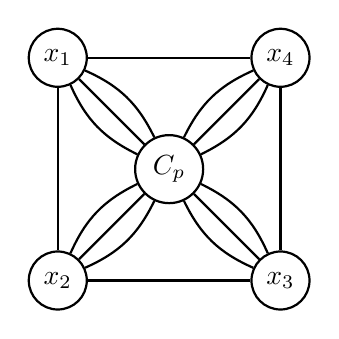
\begin{tikzpicture}[node distance={20mm}, thick, main/.style = {draw, circle}] 
        \node[main] (C) {$C_p$};
        \node[main] (1) [above left of=C] {$x_1$}; 
        \node[main] (2) [below left  of=C] {$x_2$};
        \node[main] (3) [below right of=C] {$x_3$}; 
        \node[main] (4) [above right of=C] {$x_4$};
        \draw (1) -- (2);
        \draw (2) -- (3);
        \draw (4) -- (3);
        \draw (1) -- (4);
        
        \draw (1) -- (C);
        \path[-] (1) edge [bend left=20] node {} (C);
        \path[-] (1) edge [bend right=20] node {} (C);

        \draw (2) -- (C);
        \path[-] (2) edge [bend left=20] node {} (C);
        \path[-] (2) edge [bend right=20] node {} (C);
        
        \draw (3) -- (C);
        \path[-] (3) edge [bend left=20] node {} (C);
        \path[-] (3) edge [bend right=20] node {} (C);

        \draw (4) -- (C);
        \path[-] (4) edge [bend left=20] node {} (C);
        \path[-] (4) edge [bend right=20] node {} (C);
    \end{tikzpicture}
    \caption{The graph $\G_0$ depicted here is a subgraph of the complete graph $\G$ which encodes a constant number of independence constraints as $p$ grows.}
    \label{fig-graph-exp-1}
\end{figure}

To evaluate the size of each approximation, we follow the numerical procedure used in Tang et al.\,\cite{Tang2020}. For a fixed sample size $n = 100$ and values $p = 5, 10, 20, 50, 75, 90$, we perform a series of experiments with the goal of evaluating the approximations of the respective test statistics under the null hypothesis. In each experiment, we execute the following procedure
\begin{enumerate}
    \item Sample a random precision matrix $\Omega \in \S(\G_0)$ as described in Appendix \ref{sec-precision-sampling}.
    \item Sample a set of observations $X_1, \ldots, X_n \simiid N_p(0, \Omega^{-1})$ and compute the sufficient statistic $S_n = X X^\top / n$.
    \item Compute the test statistics $\Lambda(S_n)$ and $Q(S_n)$.
    \item Compute p-values based on the asymptotic approximations to the distribution of the test statistics.
\end{enumerate}
Repeating the experiment $N = 25\ 000$ times provides a large sample of p-values for each constructed test. Under the null hypothesis, the approximate distributions are asymptotically valid, hence the p-values are asymptotically uniform on $[0, 1]$. As shown in the upper pane of Figure \ref{fig-complete-to-4cycle}, the distribution of the p-values in the likelihood ratio test is not uniform for $p \geq 10$. On the other hand, the p-values for the Erisken test appear to remain uniform even for $p$ approaching $n$.

\begin{figure}[!tbp]
    \textbf{Evaluation of tests in 4-cycle vs.\,dense setup}
    \centering
    \subfloat{
        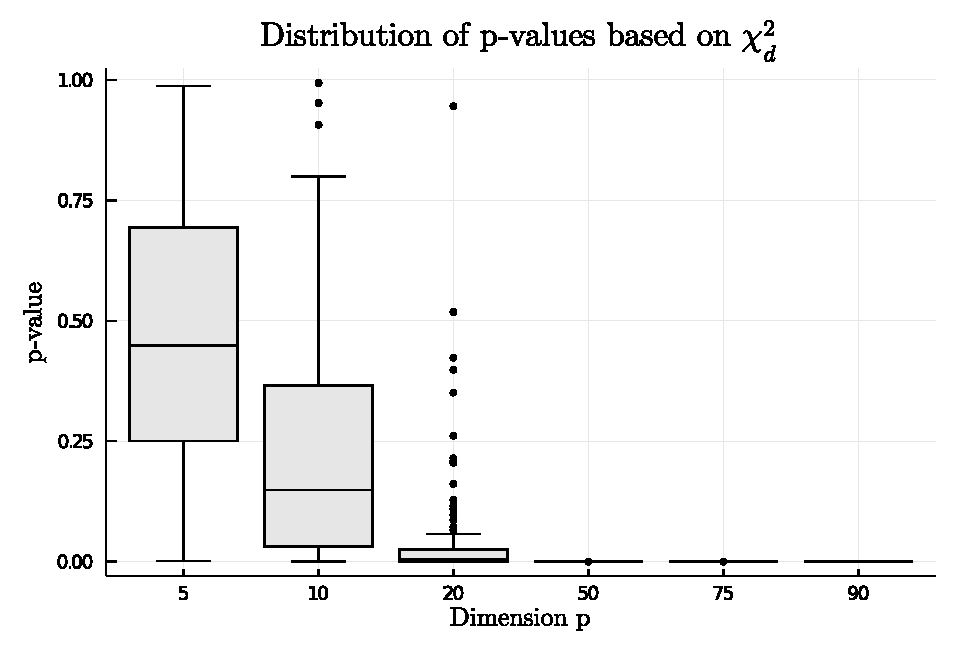
\includegraphics[width=7.5cm]{complete_to_chordless4cycle_chisq.eps}
    }
    \subfloat{
        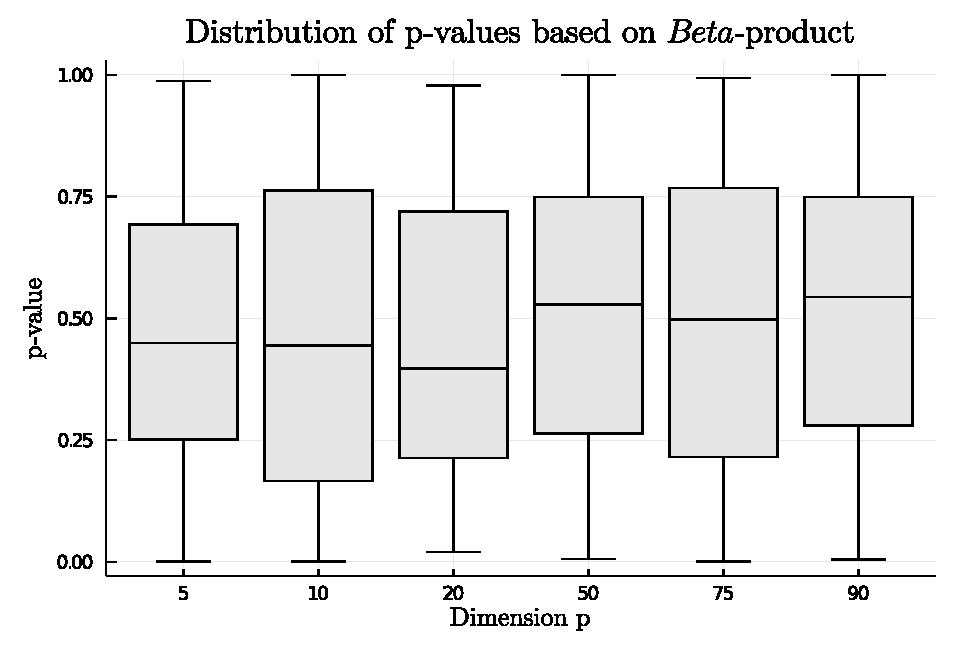
\includegraphics[width=7.5cm]{complete_to_chordless4cycle_beta.eps}
    }
    \qquad
    \subfloat{
        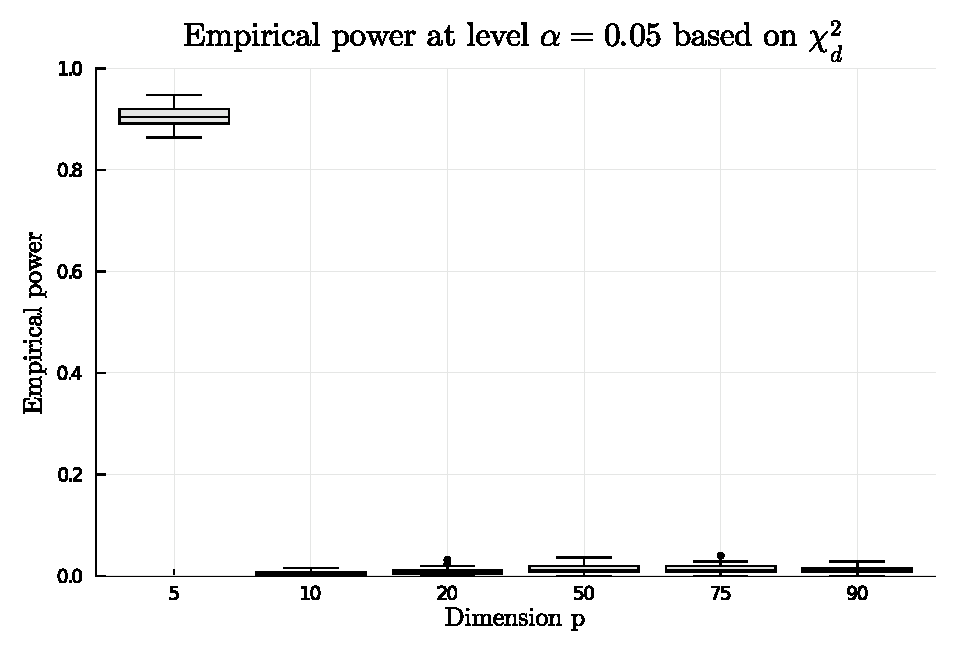
\includegraphics[width=7.5cm]{power_complete_to_chordless4cycle_chisq.eps}
    }
    \subfloat{
        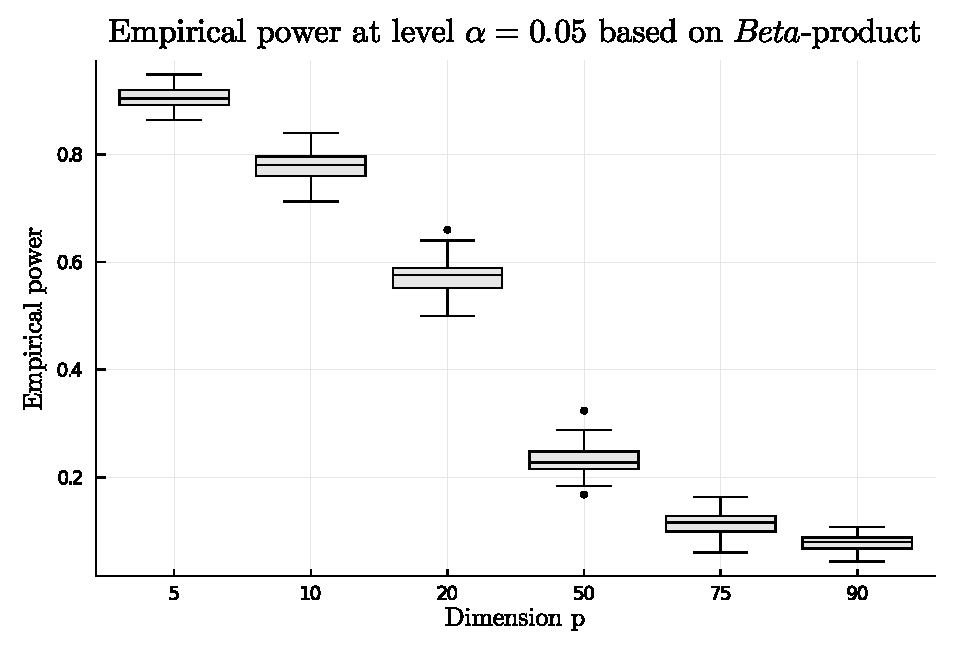
\includegraphics[width=7.5cm]{power_complete_to_chordless4cycle_beta.eps}
    }
    \caption{Evaluation of the tests based on the $\chi^2_d$ and Eriksen approximations for $n = 100$ and $p = 5, 10, 20, 50, 75, 90$. The null hypothesis corresponds to the complete graph minus two edges, forming a 4-cycle and the alternative hypothesis is the complete graph. The upper panes show the distribution of p-values when the data is sampled from the null hypothesis. The lower pane displays the Monte-Carlo estimate of the rejection rate of each test when the data is sampled from the alternative hypothesis.}
    \label{fig-complete-to-4cycle}
\end{figure}


To evaluate the power of each test, we estimate the empirical rejection rate under the alternative hypothesis given a fix nominal level $\alpha = 0.05$. Similarly to the evaluation of the size of each test, we fix the sample size $n = 100$ and perform experiments for different values of $p = 5, 10, 20, 50, 75, 90$. For estimating the power of a test, we adapt step 1 of the experiment described above with sampling $\Omega$ from the alternative hypothesis instead of the null hypotheses to have $\Omega \in \S_{\succ 0}(\G) \setminus \S_{\succ 0}(\G_0)$. With a sample of $N = 25\ 000$ p-values from each test, we compute the Monte-Carlo estimate of the average test power at level $\alpha = 0.05$ by dividing the number of p-values falling under this threshold by $N$. We visualize these results in the lower pane of Figure \ref{fig-complete-to-4cycle}, in which we can see that both tests suffer from a strong loss of power as the number of nodes in the graph grows.


Next, we consider a second setup, in which the number of edges removed from $\G$ to form $\G_0$ grows with the number of nodes in $\G$. We define $\G$ to be a complete graph over $p$ nodes and $\G_0$ to be the $p$-cycle defined in Example \ref{ex-pcycle}. In this case, we have $p$ nuisance parameters corresponding the edges in $\G_0$ and we have $p(p-1)/2$ parameters of interest corresponding to the edges removed from $\G$. Further, in this setup, $d = |E| - |E_0| = p(p-1)/2 - p = p(p-3)/2$. Hence $\Lambda(S_n)$ is asymptotically $\chi^2_{p(p-3)/2}$. The Eriksen approximation to the distribution of $Q(S_n)$ is a product of $p(p-3)/2$ random variables following Beta distributions. To compute the parameters of these Beta distributions, we iteratively remove edges from $\G$ following a lexicographical ordering: $\eset{1, 3}, \eset{1, 4}, \ldots, \eset{1, p-1}, \eset{2, 4}, \ldots, \eset{2, p}, \eset{3, 5} \ldots, \eset{p-2, p}$. For each edge removed, the graph is updated and the parameters of the corresponding Beta random variable are computed. The detailed algorithm is displayed in Algorithm \ref{alg:comp-beta}.

\begin{algorithm}[t!]
    \caption{Compute Betas for approximation of $Q(S_n)$ in $p$-cycle vs.\,complete problem}
    \label{alg:comp-beta}
    \begin{algorithmic}[1]
    \Require{Number of nodes $p$.} 
    \Ensure{Parametrized beta variables for approximating the disrtibution of $Q(S_n)$.}
        \State {Let Betas$ = \eset{}$}
        \State {Let $\G = ([p], E)$ be the complete graph over $[p]$}

        \For{$i = 1, \ldots, p-2$}
            \For{$j = i + 2, \ldots, p$}
                \If{$\eset{i, j} = \eset{1, p}$ }
                    \State{Skip iteration}
                \EndIf
                
                \State{Set $E := E \setminus\eset{\eset{i, j}}$ and $\G := ([p], E)$}

                \State{Let $C = |\t{bd}_\G(i) \cap \t{bd}_\G(j)|$ }

                \State{Set Betas = Betas $\cup\ \eset{B((n-C-1)/2, 1/2)}$}
            \EndFor
        \EndFor
        \State{Return Betas}
    \end{algorithmic}
\end{algorithm}

We evaluate the size of each test following the same procedure as in the previous setup. The result displayed in the upper pane of Figure \ref{fig-complete-to-pcycle} shows that the $\chi^2_d$ approximation only properly approximate the distribution of $\Lambda(S_n)$ under the null hypothesis when the dimension $p$ is kept low. This time however, the Eriksen approximation is only accurate for $p \leq 20$.

Similarly for the power, we use the same procedure as in the previous setup with the same nominal level $\alpha = 0.05$. While the lower pane of Figure \ref{fig-complete-to-pcycle} shows that the $\chi^2_d$ approximation suffers from the same loss of power for $p > 10$, the test based on the $Q(S_n)$ statistic has a power of 1 in every setup. This could be explained by the large difference between the null and alternative hypotheses.

\begin{figure}[!tbp]
    \textbf{Evaluation of tests in $p$-cycle vs.\,dense setup}
    \centering
    \subfloat{
        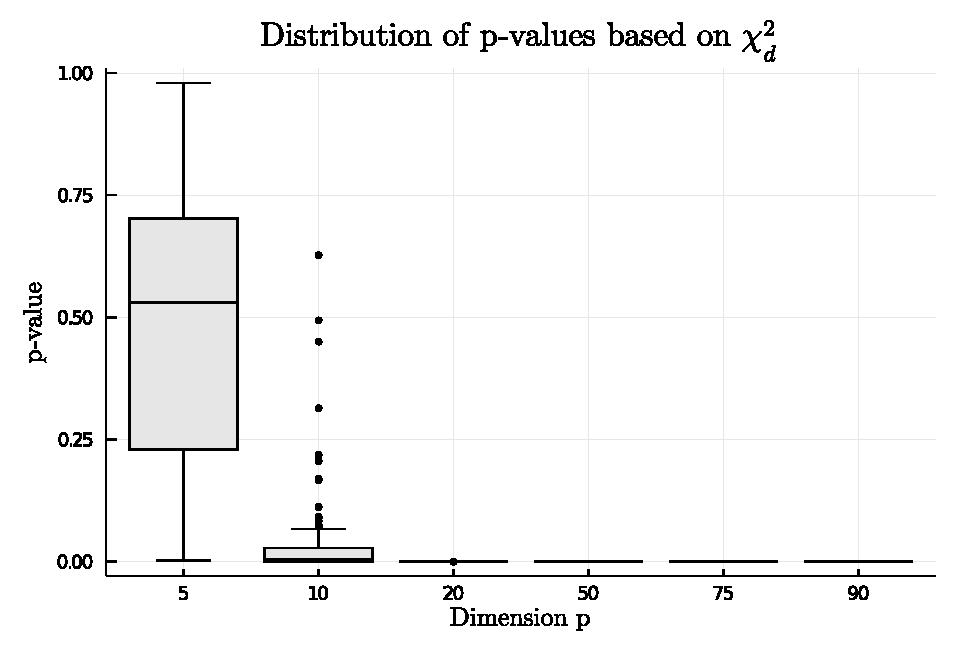
\includegraphics[width=7.5cm]{complete_to_pcycle_chisq.eps}
    }
    \subfloat{
        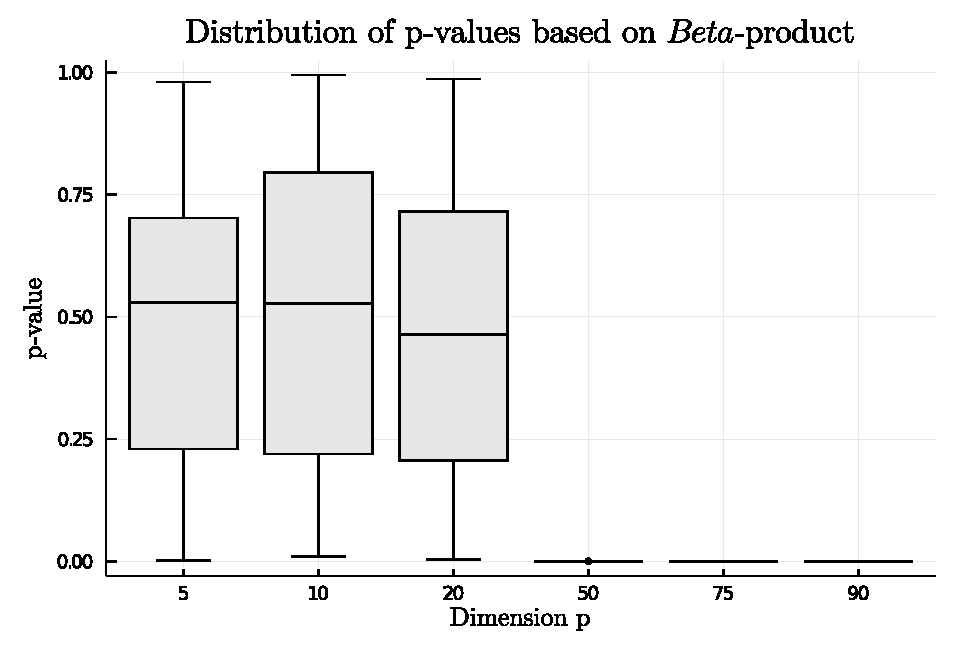
\includegraphics[width=7.5cm]{complete_to_pcycle_beta.eps}
    }
    \qquad
    \subfloat{
        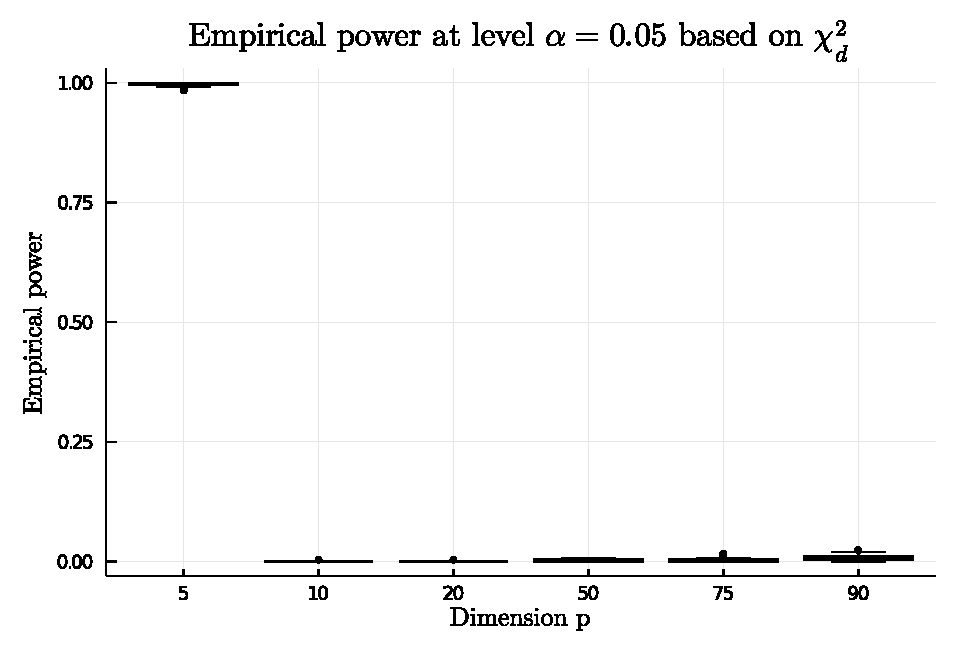
\includegraphics[width=7.5cm]{power_complete_to_cycle_chisq.eps}
    }
    \subfloat{
        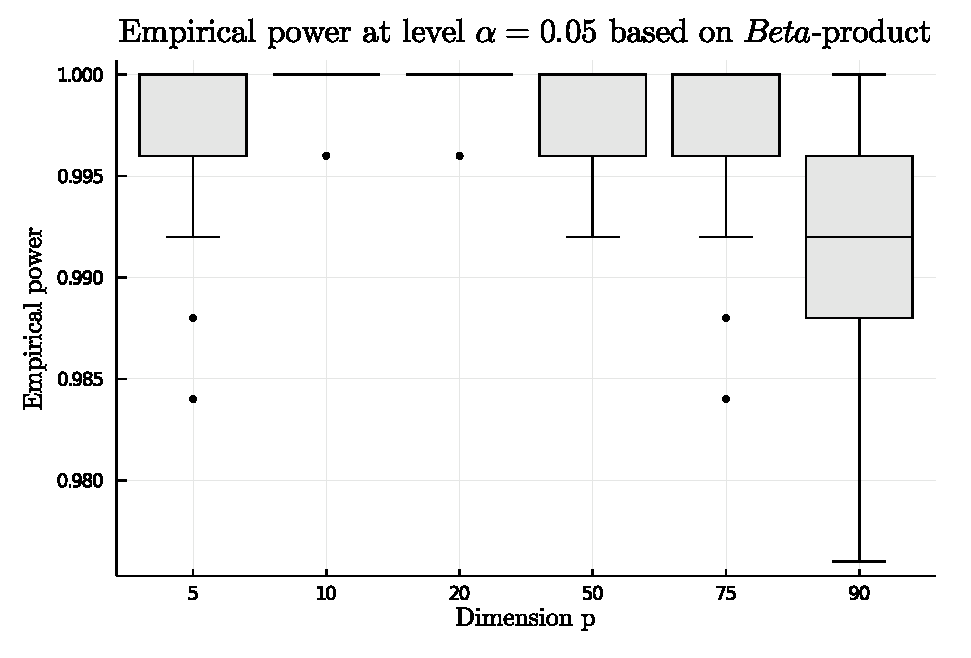
\includegraphics[width=7.5cm]{power_complete_to_cycle_beta.eps}
    }
    \caption{Evaluation of the tests based on the $\chi^2_d$ and Eriksen approximations for $n = 100$ and $p = 5, 10, 20, 50, 75, 90$. The upper panes show the distribution of p-values when the data is sampled from the null hypothesis. The null hypothesis corresponds to a $p$-cycle and the alternative hypothesis is the complete graph. The lower pane displays the Monte-Carlo estimate of the rejection rate of each test when the data is sampled from the alternative hypothesis.}
    \label{fig-complete-to-pcycle}
\end{figure}
